\section[Xsemantics]{Implementation in Xsemantics}

\begin{frame}
\frametitle{Xsemantics}
\tableofcontents[currentsection]

\end{frame}

\begin{frame}
\frametitle{Xsemantics}

\begin{itemize}
  \item  a DSL for writing 
  \begin{itemize}
    \item type systems (static semantics)
    \item reduction rules (dynamic semantics)
    \item interpreters
    \item general relation rules
  \end{itemize}
  for languages implemented in Xtext
  \item A system definition is a set of judgment rules which have a
conclusion and a set of premises (relying on Xbase for the syntax)
  \item thought to be used by people who are familiar
with formal type systems and operational semantics
  \item aims at providing
a syntax which is close to the way deduction rules are written in a formal
setting
\end{itemize}

\end{frame}

\begin{frame}
\frametitle{Define your judgments}

\begin{footnotesize}
% Generator: GNU source-highlight, by Lorenzo Bettini, http://www.gnu.org/software/src-highlite
\begin{tabular}[t]{l}
\noindent
\mbox{}\textbf{\textcolor{Plum}{system}}\ org.typesys.xsem.guidsl.xsemantics.TypeSystem \\
\mbox{} \\
\mbox{}\textbf{\textcolor{Plum}{import}}\ org.typesys.xsem.guidsl.xsemGuiDsl.* \\
\mbox{} \\
\mbox{}\textbf{\textcolor{Plum}{judgments}}\ \{ \\
\mbox{}\ \ \ \ type\ $|$-\ Typable\ typable\ :\ \textbf{\textcolor{Plum}{output}}\ Type \\
\mbox{}\ \ \ \ \textcolor{Green}{//\ whether\ \{@code\ right\}\ is\ assignable\ to\ \{@code\ left\}} \\
\mbox{}\ \ \ \ isAssignable\ $|$-\ Type\ left\ $<$$\sim$\ Type\ right \\
\mbox{}\ \ \ \ \textcolor{Green}{//\ computes\ the\ most\ general\ type\ between\ \{@code\ first\}\ and\ \{@code\ second\}} \\
\mbox{}\ \ \ \ mostGeneral\ $|$-\ Type\ first\ $\sim$$\sim$\ \ Type\ second\ $|$$>$\ \textbf{\textcolor{Plum}{output}}\ Type \\
\mbox{}\}
\end{tabular}

\end{footnotesize}

\end{frame}


\begin{frame}
\frametitle{Similarities}

\begin{center}
\begin{tabular}{c@{\hspace{1cm}}c}
\inferrule
{}
{\g \f \mykeyb{true} : \mykeyb{boolean} }
&
\inferrule
{\g \f \mytt{attr} : \T}
{\g \f \mykeyb{ref} \ \mytt{attr} : \T }
\end{tabular}
\end{center}

\onslide<2->

\begin{footnotesize}
% Generator: GNU source-highlight, by Lorenzo Bettini, http://www.gnu.org/software/src-highlite
\begin{tabular}[t]{l}
\noindent
\mbox{}\textbf{\textcolor{Plum}{axiom}}\ BooleanLiteralType \\
\mbox{}\ \ \ \ G\ $|$-\ BooleanLiteral\ lit\ :\ XsemGuiDslFactory::eINSTANCE.createBooleanType \\
\mbox{} \\
\mbox{}\textbf{\textcolor{Plum}{rule}}\ AttributeRefType \\
\mbox{}\ \ \ \ G\ $|$-\ AttributeRef\ attrRef\ :\ Type\ type \\
\mbox{}\textbf{\textcolor{Plum}{from}}\ \{ \\
\mbox{}\ \ \ \ G\ $|$-\ attrRef.attr\ :\ type \\
\mbox{}\}
\end{tabular}

\end{footnotesize}

\end{frame}

\begin{frame}
\frametitle{Similarities}

\begin{center}
\begin{tabular}{c@{\hspace{.5cm}}c@{\hspace{.5cm}}c}
\inferrule
{\g \f \mytt{exp} : \mykeyb{string}}
{\g \f \mykeyb{lengthOf}(\mytt{exp}) : \mykeyb{int} }
&
\inferrule
{\g \f \g(\mykeyb{widgetcontent}) : \T}
{\g \f \mykeyb{widgetcontent} : \T }
\end{tabular}
\end{center}

\onslide<2->

\begin{footnotesize}
% Generator: GNU source-highlight, by Lorenzo Bettini, http://www.gnu.org/software/src-highlite
\begin{tabular}[t]{l}
\noindent
\mbox{}\textbf{\textcolor{Plum}{rule}}\ LengthOfType \\
\mbox{}\ \ \ \ G\ $|$-\ LenghtOf\ len\ :\ XsemGuiDslFactory::eINSTANCE.createIntType \\
\mbox{}\textbf{\textcolor{Plum}{from}}\ \{ \\
\mbox{}\ \ \ \ G\ $|$-\ len.expr\ :\ \textbf{\textcolor{Plum}{var}}\ StringType\ stringType \\
\mbox{}\} \\
\mbox{} \\
\mbox{}\textbf{\textcolor{Plum}{rule}}\ FieldContentType \\
\mbox{}\ \ \ \ G\ $|$-\ FieldContent\ fieldContent\ :\ Type\ type \\
\mbox{}\textbf{\textcolor{Plum}{from}}\ \{ \\
\mbox{}\ \ \ \ G\ $|$-\ \textbf{\textcolor{Plum}{env}}(G,\ \textcolor{RoyalBlue}{'widgetcontent'},\ Attribute)\ :\ type \\
\mbox{}\}
\end{tabular}

\end{footnotesize}

\end{frame}


\begin{frame}
\frametitle{The generated validator}

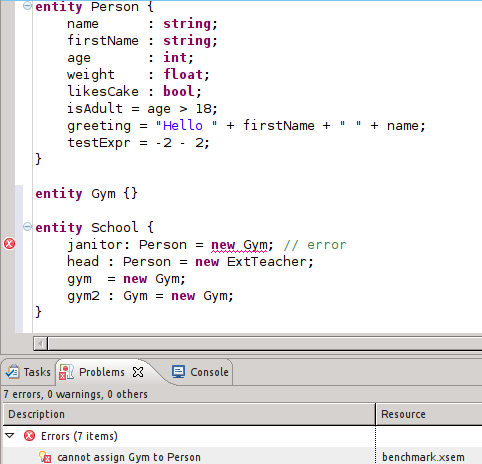
\includegraphics[width=.7\textwidth]{img/xsem-validation.png}

\end{frame}

\begin{frame}[fragile]
\frametitle{Traces}

\begin{itemize}
  \item Automatic trace generation:
  \begin{itemize}
    \item for rule sucessful applications
    \item for rule failures
  \end{itemize}
  \item Useful for testing and debugging
\end{itemize}

\medskip

\begin{footnotesize}
\begin{verbatim}
final result provided by rule MyRule
 rule 1 used by MyRule to get to the result
  rule 2 used by rule 1
   rule 3 used by rule 2
   ...
 rule 1a used by MyRule to get to the result
  rule 2a used by rule 1a
  ...
\end{verbatim}
\end{footnotesize}

\end{frame}

\begin{frame}
\frametitle{A tool for the ``formal'' designer}

\begin{itemize}
  \item Write the theory of a language
  \begin{itemize}
    \item Write the type system
    \item Write the semantics
    \item Prove that the latter is consistent with the former
  \end{itemize}   
  \item With Xtext you can develop a quick prototype
  \item With Xsemantics you can smoothly encode the formal system
  in the implementation
  \item Help in filling the gap between the theory and the implementation
\end{itemize}

\end{frame}